\documentclass[11pt]{article}
\usepackage[czech]{babel}
\usepackage[utf8]{inputenc}
\usepackage{graphicx}
%% \usepackage{a4wide}

\newcommand\CARET{\mathbin{\char`\^}}


\title{Vizualizace grafu matematické funkce}
\author{Tomáš Maršálek}
\date{\today}

\begin{document}
\maketitle

\section{Zadání}
Naprogramujte v ANSI C přenositelnou1 konzolovou aplikaci, která jako vstup
načte z parametru na příkazové řádce matematickou funkci ve tvaru $y = f(x)$,
provede její analýzu a vytvoří soubor ve formátu PostScript s grafem této
funkce na zvoleném definičním oboru.

\section{Analýza úlohy}
Abychom mohli zobrazit graf funkce jako například x $\CARET$ 2 + sin(x), musíme
být nejdříve schopni vyhodnotit tuto funkci numericky. Tedy musíme ve výrazu
rozpoznat jednotlivá čísla, proměnné nebo operátory a rozpoznat jejich význam.
Standardním postupem při parsování vstupního řetězce je rozdělení úlohy na
několik po sobě následujících částí tak, aby se případné chyby ve vstupu
odhalily v příslušné části a nepropagovaly se do následující. Každá část
se tedy stará pouze o chyby, které se jí týkají.

\subsection{Lexikální analýza}
Místo abychom při vyhodnocování výrazu postupně hledali čísla nebo operátory,
ponecháme tuto úlohu specializovanému nástroji, takzvanému scanneru nebo také
lexeru.  Nadefinujeme jednotlivé symboly a necháme scanner, aby je ve vstupním
řetězci rozpoznal, nebo aby případně rozpoznal lexikální chyby.  Význam celé
této fáze je v zjednodušení nadcházející fáze, která je složitější, a už se
nebude muset zabývat problémy typu jestli je symbol skutečně číslo nebo jestli
symbol \uv{sin} je ve skutečnosti \uv{sinh} a podobně.

\subsection{Syntaktická a sémantická analýza}
Tyto dvě fáze jsou zde kombinované v jednu. Vytvoříme přeloženou datovou
strukturu, se kterou bude vyhodnocování výrazu víceméně triviální. Syntaktická
analýza najde chyby týkající se skladby výrazu, jako například dvě čísla nebo
znaky následující po sobě, chybějící závorky, a podobně. Jednotlivým symbolům
přiřadíme jejich význam, tj. číslům jejich numerickou hodnotu a operátorům
jejich příslušnou unární nebo binární funkci. 

\subsection{Postfixová notace}
Výsledná datová struktura je posloupnost symbolů v postfixové nebo také
reverzní polské notaci. Výhoda tohoto zápisu oproti klasické infixové notaci
je absence závorek a jednoduchost vyhodnocení výrazu. Při vyhodnocování totiž
vždy když narazíme na operátor, máme jistotu, že všechny předcházející znaky, 
které operátor vyžaduje, jsou čísla.

Příklad infixové a postfixové notace.
\begin{center}
\begin{tabular}{|l|l|}
\hline
infix & postfix \\
\hline
1 + 1 & 1 1 + \\
1 + 2 * 3 & 1 2 3 * + \\
(1 + 2) * 3 & 1 2 + 3 * \\
x * $\sin$ (x $\CARET$ 2) & x x 2 $\CARET$ $\sin$ * \\
1 - 2 - 3 + 4 $\CARET$ 5 $\CARET$ 6 & 1 2 - 3 - 4 5 6 $\CARET$ $\CARET$ + \\
\hline
\end{tabular}
\end{center}

Metoda na převedení infixového do postfixového zápisu je např. Dijkstrův
Shunting yard algoritmus.


\subsection{Shunting yard}
Při konverzi musíme mít na paměti přednosti jednotlivých operátorů. Výraz
$1 + 2 * 3$ se musí přeložit jako $1~2~3~*~+$ a ne jako $1~2~+~3~*$.  Dále také
levou nebo pravou asociaci nekomutativních operátorů, pokud ve výrazů chybí
závorky.  Například operátor odčítání upřednostňuje levé uzávorkování ($1 - 2 -
3 = ((1 - 2) - 3)$) oproti umocňování, které naopak upřednostňuje uzávorkování
zprava ($2~\CARET~3~\CARET~4 = (2~\CARET~(3~\CARET~4)) = 2^{3^4}$).

Algoritmus používá pomocný zásobník na odkládání operátorů, dokud nemá jistotu
o jejich správném umístění v postfixu. Čteme infixový výraz zleva doprava po
jednotlivých symbolech a vždy když narazíme na symbol typu číslo nebo proměnná,
pouze ho uložíme do výsledné výstupní fronty. Pokud narazíme na operátor,
všechny operátory, které dosud leží nahoře v zásobníku a vážou se těsněji (mají
vyšší precedenci) než právě vytažený symbol, můžeme přidat do výsledné fronty.
Právě vytažený symbol pak pouze vložíme na zásobník. Až nám dojdou všechny
symboly, pouze vytáhneme všechny operátory ze zásobníku a v tomto pořadí je
přidáme do výsledné fronty. \\

Jako příklad mějme výraz 1 / 2~$\CARET$~3 + 4.
\begin{center}
\begin{tabular}{|c|l|l|r|}
\hline
symbol & výsledek & zásobník & akce \\
\hline
1 & 1 & & číslo, pouze přidáme do fronty \\
/ & 1 & / & dosud žádný operátor v zásobníku\\
2 & 1 2 & / & číslo, pouze přidáme do fronty \\
$\CARET$ & 1 2 & / $\CARET$ & / má slabší vazbu než $\CARET$, necháme být \\
3 & 1 2 3 & / $\CARET$ & číslo, pouze přidáme do fronty \\
+ & 1 2 3 $\CARET$ / & + & $\CARET$ a / mají silnější vazbu než + \\
4 & 1 2 3 $\CARET$ / 4 & + & číslo, pouze přidáme do fronty \\
konec  & 1 2 3 $\CARET$ / 4 + & & konec, přidáme všechny operátory \\

\hline
\end{tabular}
\end{center}

\subsection{Zobrazení grafu}
Jednoduchým řešením jak zobrazit funkci je vyhodnotit vždy dva sousední body a
spojit je úsečkou. Důležité je pouze zvolit dostatečně detailní rozdělení osy
x, aby graf nebyl kostrbatý.

Úsporná metoda, která řeší kostrbatost zobrazené funkce je adaptivní
vyhlazování. Šetření zobrazenými přímkami oceníme zejména u jednoduchých
funkcí, protože rozhodně nepotřebujeme, aby graf funkce $f(x) = x$ byl stejně
detailní jako graf funkce $f(x) = sin(1/x)$, který je kolem nuly velmi
detailní. Taktika je poměrně jednoduchá.  Mějme zvolené nějaké počáteční
rozdělení osy x a pokud při zobrazování jednotlivých úseček zjistíme, že by
došlo k příliš velkému skoku ve sklonu dvou sousedních úseček (výpočetně by
druhá diference přesahovala jistý zvolený práh), rozdělíme interval mezi $x_i$
a $x_{i + 1}$ na polovinu. Samozřejmě musíme mít nějaký limit tohoto půlení,
protože u funkcí typu $f(x) = sin(1/x)$ by došlo kolem nuly k nekonečnému
půlení. Stejným výpočtem se snažíme zajistit co nejdelší interval, abychom
zbytečně neplýtvali úsečkami. 

\begin{figure}[ht!]
\centering
	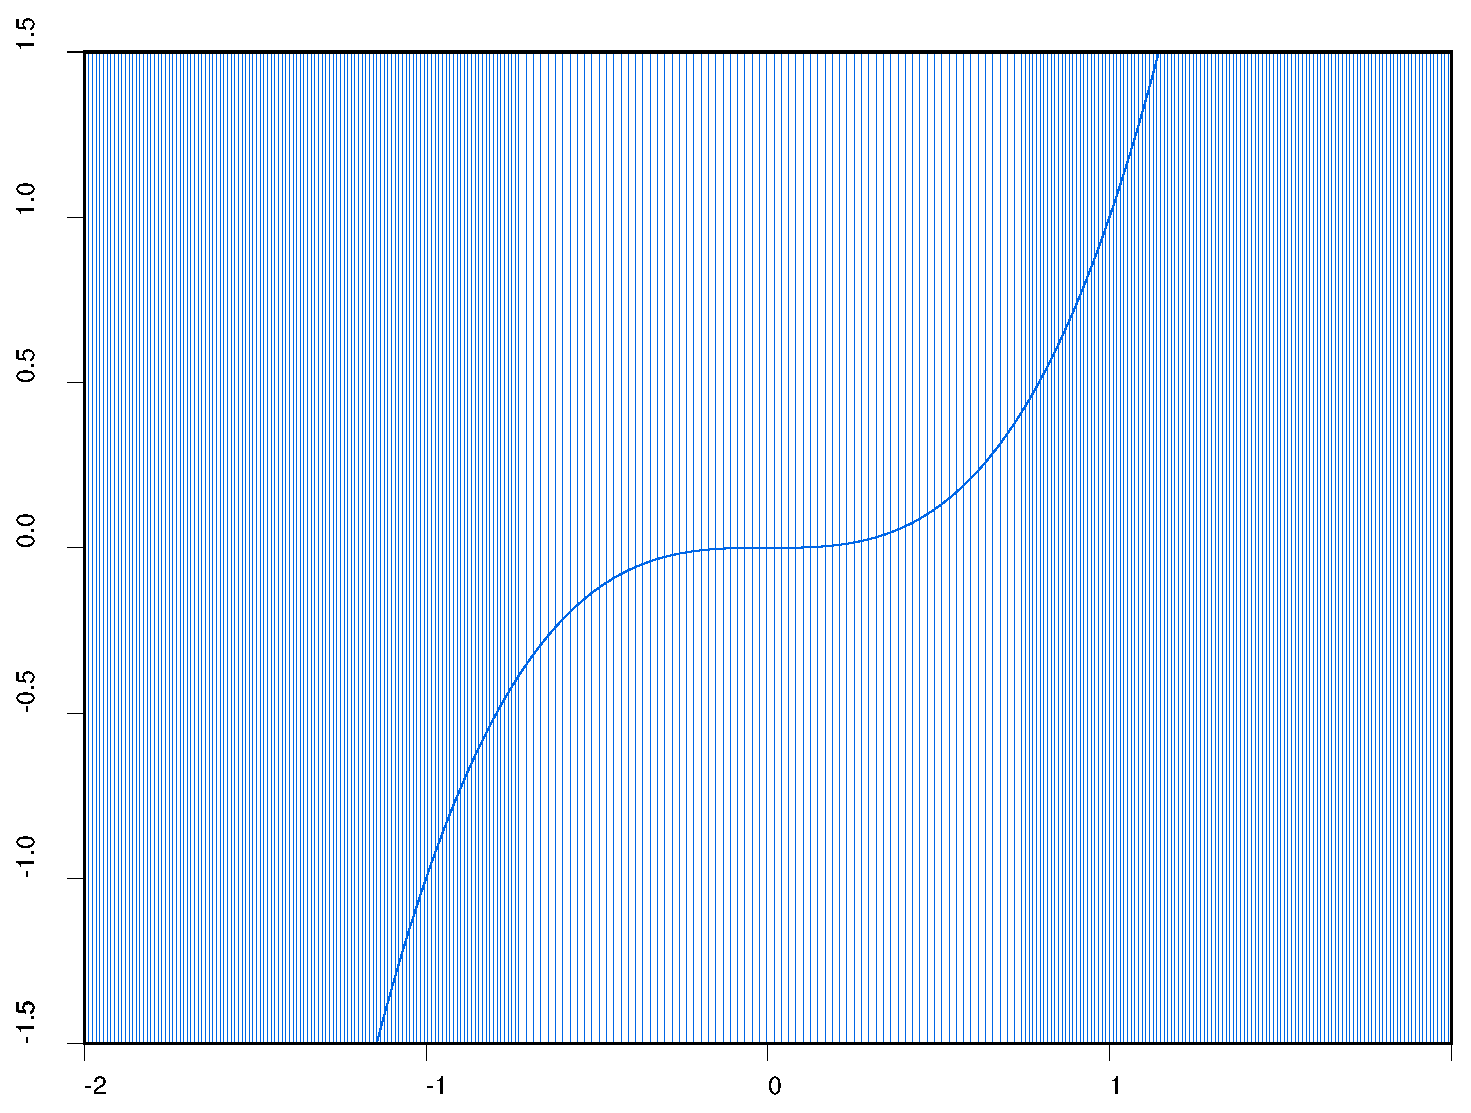
\includegraphics[width=11cm]{figures/figure2.eps}
	\caption{Rozdělení osy x grafu funkce $x^3$}
\end{figure}
\begin{figure}[ht!]
\centering
	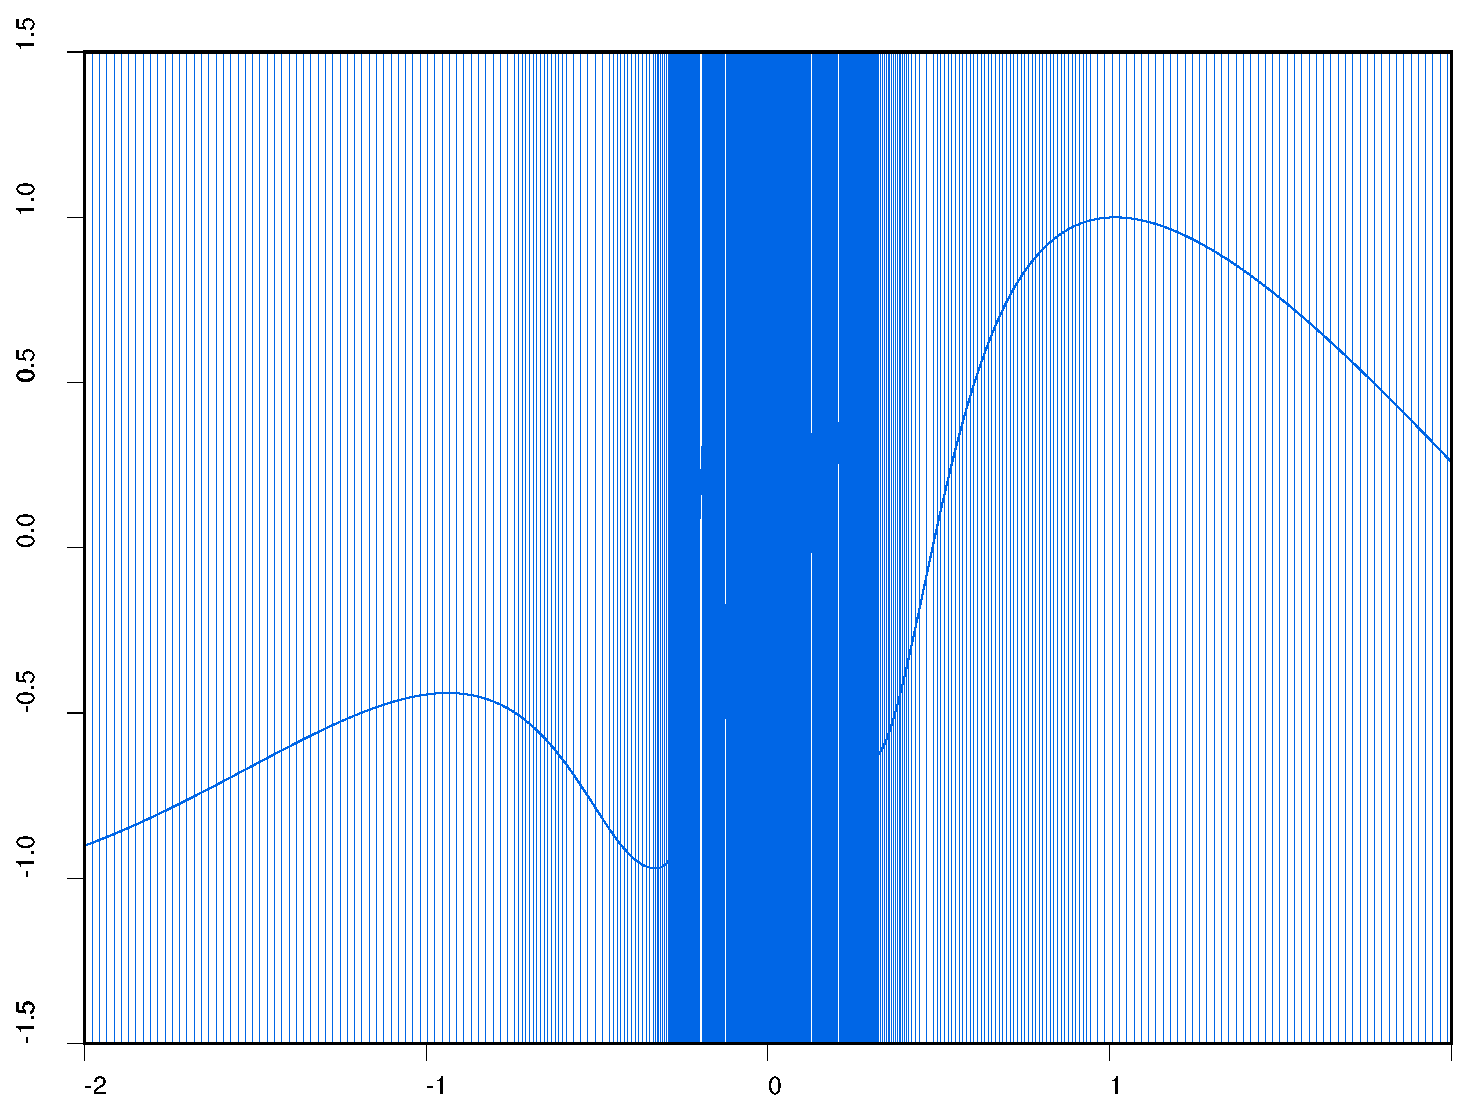
\includegraphics[width=11cm]{figures/figure1.eps}
	\caption{Rozdělení osy x grafu funkce
		$\sin \left(x + \cos \left(\frac{1}{x} \right) \right)$}
\end{figure}

\clearpage
Zřejmým problémem jsou funkce, které v některých bodech zadaného intervalu
rostou limitně do nekonečna, případně nejsou na daném intervalu definovány.
Případ, kdy funkce pokračuje mimo zadanou hranici, případně až do nekonečna je
celkem jednoduchý. Aby nedošlo k useklým grafům poblíž dolní nebo horní
hranice, stačí vypočítat průsečík horní nebo dolní hranice s úsečkou mezi
posledním bodem a bodem, který už by byl mimo graf a vést kratší úsečku do
tohoto průsečíku. 

Horší jsou funkce, které nejsou definovány v určitém místě. Implementace
těchto funkcí v matematické knihovně v takových případech vracejí hodnotu NaN.
Výpočet průsečíku s takovým číslem nedává smysl a předefinování knihovních
funkcí na vlastní, které by vracely alespoň nekonečna namísto NaN způsobuje
jiné nežádoucí artefakty. Například předefinování logaritmů pro záporné hodnoty
na záporné nekonečno funguje dokud nezobrazíme nějakou transformaci tohoto
logaritmu na reálné hodnoty (např. $f(x) = exp(ln(x))$). Pro jednoduchost je
tedy možná lepší NaN hodnoty pouze nezobrazovat.

%% TODO nekonecno figure


\section{Implementace}
\paragraph{Lexer} 
je konstruován jako deterministický automat, který rozpoznává celá čísla v
šestnáctkové, desítkové a osmičkové soustavě, floating point čísla, proměnnou
x, operátory a závorky. Mezery rovnou zahazuje. V případě chyby posílá chybový
token do další fáze.  Token je zde struktura, která si uchovává pozici a délku
nalezeného podřetězce a samotný řetězec pro případný výpis chyby.

\paragraph{Parser}
je implementace Shunting yard algoritmu, která navíc kontroluje syntaktické
chyby. Výsledek je vrácen jako posloupnost symbolů, které ale musí být po
skončení používání dealokovány. Pro zjednoduššení jsou všechny tokeny a
přeložené symboly uchovány v pomocných polích, aby na konci došlo k jejich
bezchybnému dealokování. Symbol je výsledný přeložený token, který je zde
implementován jako polymorfní struktura (uchovává si svůj typ a případně data
vztahující se k jednotlivým typům). Mohla by být implementována i efektivněji,
například pomocí $union$, ale v ANSI C není podporován anonymní $union$. S
pojmenovaným by zdrojový kód vypadal poněkud těžkopádně a navíc k příliš
velkému ušetření paměti by rozhodně nedošlo. Zvolil jsem tedy raději čitelnost
kódu. 

Pomocnou datovou strukturu zde tvoří pouze zásobník, který se využívá při
Shunting yard algoritmu a poté při kontrolním průchodu výsledným postfixovým
výrazem, kdy se potvrdí, že výraz bude skutečně možné vyhodnotit. Zde se odstraní chyby související s n-aritou operátorů.

\paragraph{Zobrazení grafu}
je zajištěno dalším odděleným modulem. Ten nejprve zkonstruuje hlavičku
postscriptového souboru podle specifikace postscriptu. 

Poté je funkce vyhodnocena v klíčových bodech, které jsou poté transformovány
na souřadnice postscriptového formátu stránky a spojeny úsečkami tak, jak bylo
popsáno v analýze úlohy. 

Dalším krokem je vytvoření rámečku grafu a pro přehlednost rozdělení obou os.
Velikost jednotlivých dílků je vybrána tak, aby rozdělení osy nebylo příliš
husté ani řídké, a podle konvence, že dílky mají velikost pouze 1, 2 nebo 5
krát mocnina deseti.

Nakonec jsou zapsány závěrečné postscriptové komentáře a soubor je uzavřen.


Volitelný parametr popisující defiční obor a obor hodnot je analyzován stejným
lexerem, ale má vlastní parsovací funkci.


\section{Závěr}
\end{document}
